\newpage
\section{Rendering Process}
Although the rendering process was briefly discussed in a previous section, the exact details may differ depending on used technology and implementation. This section is a step by step presentation of the rendering process in TSEngine.\\
\begin{figure}[H]
  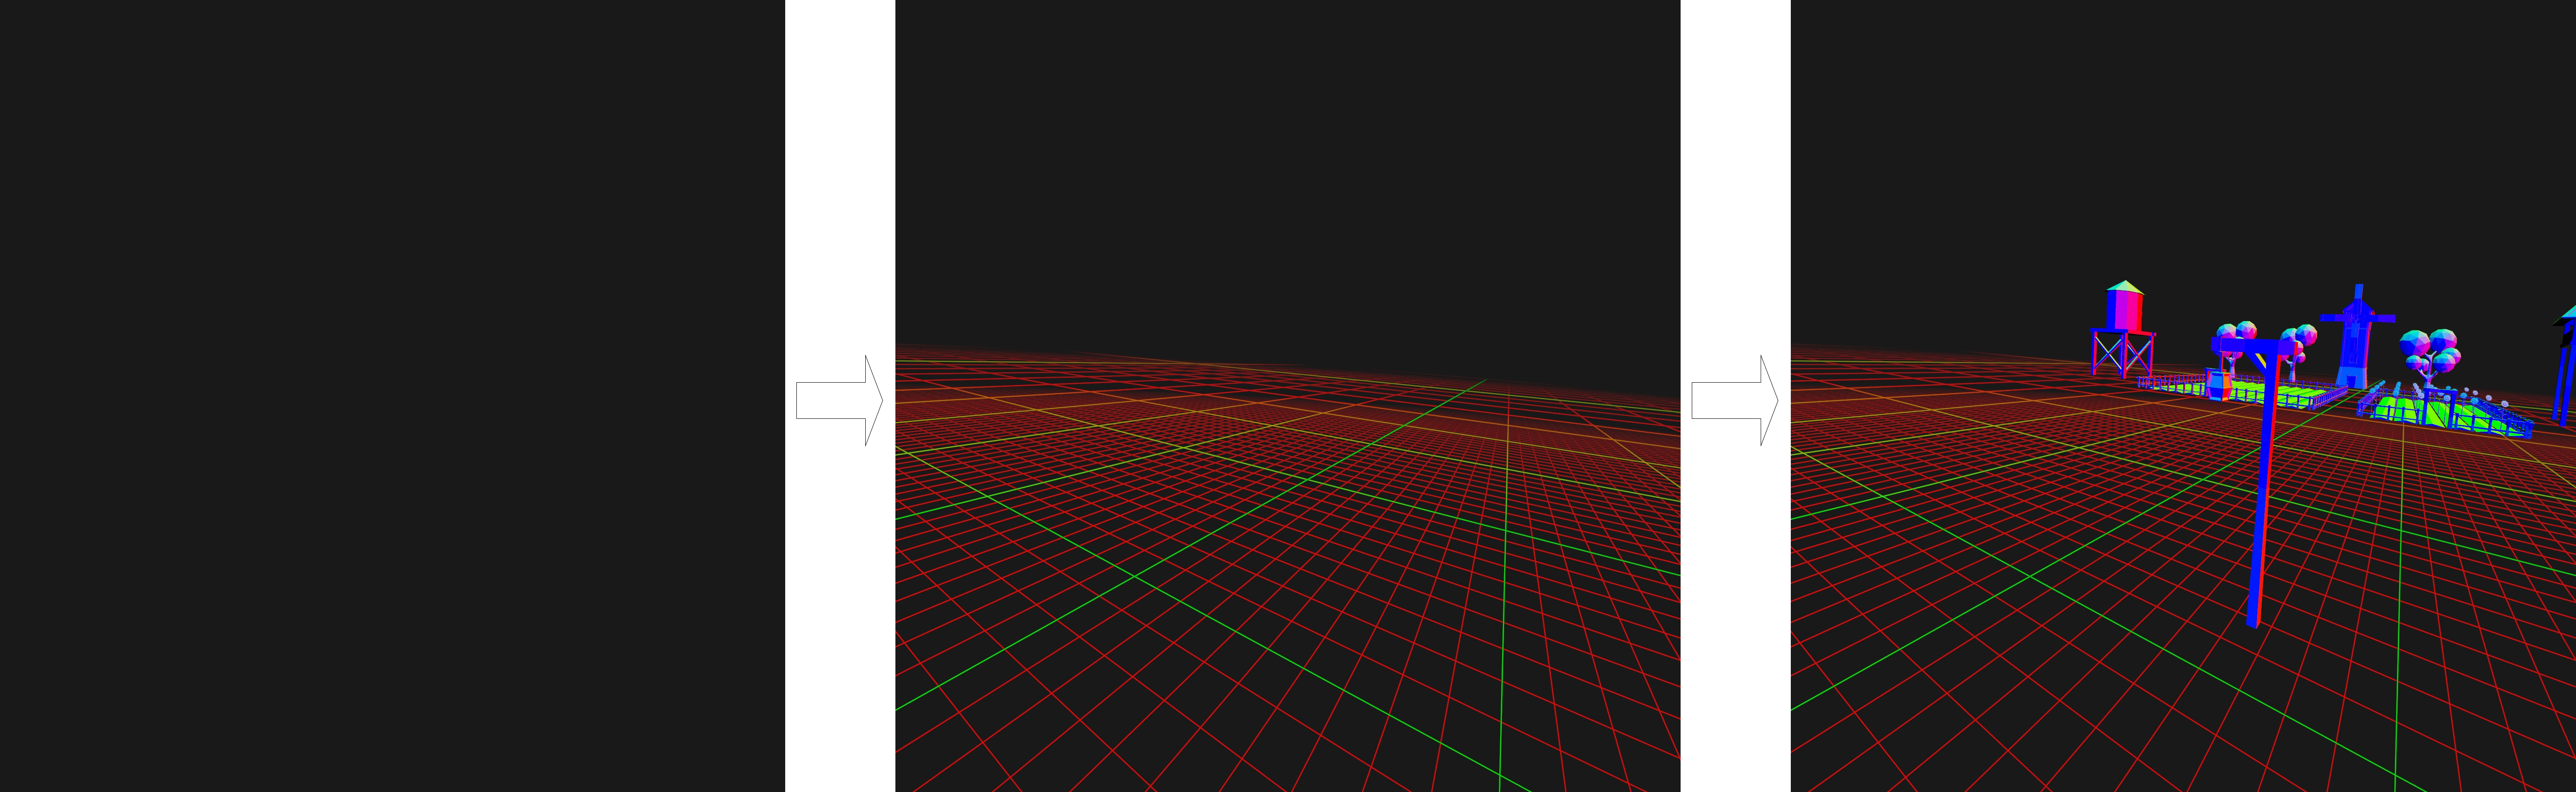
\includegraphics[width=\linewidth]{frame_generation/part1-3.png}
  \caption{Rendering process parts 1-3}
\end{figure}
In the first step, one can see an empty frame. It, as well as all others shown in this section, are consecutive framebuffers stored in RAM memory.
Secondly, the predefined grid is rendered.
In the next steps, TSEngine loads all .obj files. Order in which it does so, depends on the order directly in code, in this case the first loaded image is the village model \cite{VillageModel}



\begin{wrapfigure}{r}{0.6\textwidth}
  \includegraphics[width=\linewidth]{frame_generation/part10.jpg}
  \caption{Rendering process part 10}
\end{wrapfigure}